\documentclass[12pt]{article}
\usepackage{common}
\usepackage{appendix}
\title{Topological Significance of the Crystal Momentum}
\author{Abhirup Mukherjee}
\begin{document}
\maketitle
\subsection*{Bloch's theorem}
In the presence of a periodic potential, the plane waves get modified simply through a modulation:
\beq
\psi_{k,n}(x) = e^{i k\cdot x} u_{k,n}(x), \quad\text{where}\quad u_{k,n}(x) = u_{k,n}(x + a)
\eeq
Alternatively,
\begin{equation}\begin{aligned}
	\label{Bloch}
	\psi_{k,n}(x + a) = e^{i k a} \psi_{k,n}(x)
\end{aligned}\end{equation}
\begin{itemize}
	\item \(k\) is called the crystal momentum, and is a good quantum number of the system of free electrons in a periodic potential.
	\item It is not the canonical momentum. The canonical momentum is not conserved (because of the loss of the continuum translational symmetry).
	\item \textit{The crystal momentum acts like a center-of-mass degree of freedom for the system; just as the equation of motion for a system of particles in the presence of an external force is given by \(\frac{\:\mathrm{d}p}{\:\mathrm{d}t} = F\), the equation of motion for the electrons in a crystal under an external force is given by \(\hbar \frac{\:\mathrm{d}k}{\:\mathrm{d}t} = F\).}
\end{itemize}

\subsection*{Energy of lowest band}
Let \il{V(x)} be a periodic 1-dimensional potential in which particles of mass \il{m=1} are moving.
\beq
V(x+a) = V(x)
\eeq
We can move the coordinate axes such that it's minima are at \il{x=na}, which we take to be 0 (\il{V(na) = 0}). Then, expanding \il{V(x)} about the minimum at \(x=0\) gives
\beq
V(x) = \fr{1}{2}\omega^2 x^2 + O(x^3)
\eeq
In the approximation that the second order term dominates over the rest, the local energies are given by \(E_0 = \frac{1}{2}\hbar \omega\). If weak tunneling is allowed, the degeneracy will then be broken. The degenerate levels will split into bands. Each band forms a tight-binding model, which in second-quantized notation is
\beq
H = E_0 -t\sum_j \rr{c^\dagger_j c_{j+1} + c^\dagger_{j+1} c_{j}}
\eeq
The energies for this lowest band are
\beq
E_k = \fr{1}{2}\hbar\omega + 2t \cos ka
\eeq
The goal is to derive this last result using instantons.
\subsection*{Imaginary time and path integrals}
To do that, we will derive an expression for the probability of tunneling from one minimum to the adjacent one, between times \(t=-\frac{1}{2}T\) and \(t=\frac{1}{2}T\):
\beq
\mathcal{P}(t=-\fr{T}{2},x=0 \ra t=\fr{T}{2},x=a) = \bra{x=a} e^{-i\fr{T}{\hbar}H} \ket{x=0} = \sum_n e^{-iT E_n}\braket{x=a|n}\braket{n|x=0}
\eeq
\(\ket{n}\) are the energy eigenstates with energy \(E_n\). \textit{To extract the lowest energy from the summation, we switch to an exponentially decaying summation by introducing the Euclidean time: \il{\tau = iT}.}
\beq
\mathcal{P}(t=-\fr{T}{2},x=0 \ra t=\fr{T}{2},x=a) = \sum_n e^{-\tau E_n}\braket{x=a|n}\braket{n|x=0}
\eeq
Taking the limit of \(\tau \to \infty\) should then make just the lowest eigenvalue survive in the summation.
\begin{equation}\begin{aligned}
	\label{sasageyo}
	\mathcal{P}(t=-\infty,x=0 \ra t=\infty,x=a) = \lim_{\tau \to \infty}\sum_n e^{-\tau E_n}\braket{x=a|n}\braket{n|x=0}
\end{aligned}\end{equation}
An equivalent expression can be derived by evaluating the inner product \(\bra{2\pi} e^{-\fr{\tau}{\hbar}H} \ket{0}\) in an alternative fashion.  The process is the same one as used in deriving the path integral form of the propagator. The details are shown in the appendix. The final result is
\beq
\bra{x=a} e^{-\fr{\tau}{\hbar}H} \ket{0} &= \int\mathcal{D}\qq{x(\tau^\prime)}\ex{-\fr{S_E\qq{x(\tau^\prime)}}{\hbar}}
\eeq
where \il{S_E\qq{x(\tau^\prime)} = \int_{-\fr{\tau}{2}}^{\fr{\tau}{2}} d\tau^\prime \cc{\fr{1}{2}\dot x^2 + V(x)}} is the Euclidean action and the integration \(\int\mathcal{D}\qq{x(\tau^\prime)}\) is over all paths \(x(\tau^\prime)\) that satisfy \(x(-\frac{\tau}{2}) = 0\) and  \(x(\frac{\tau}{2}) = a\). Comparing this equation and eq.~\ref{sasageyo}, we get our main equation
\beq
\sum_n \avg{2\pi|n} e^{-\fr{\tau}{\hbar}E_n} \avg{n|0} = \int \mathcal{D}\qq{x(\tau^\prime)}\ex{-\fr{S_E}{\hbar}}
\eeq
\subsection*{The saddle point approximation and introduction of the instantons}
We will evaluate this integral by invoking the saddle point approximation:
\beq
\int \mathrm{dx} e^{f(x)} \approx \int dx \ex{f(x_0) + x^2\fr{f^{\prime\prime}(x_0)}{2}} = e^{f(x_0)}\int dx \ex{x^2\fr{f^{\prime\prime}(x_0)}{2}}
\eeq
This assumes that the majority of the contribution to \(f(x)\) comes from its minimal configuration and the quadratic fluctuations. \textit{For the present case, this involves retaining only that path \(x(\tau)\) for which the Euclidean action is a minimum, and quadratic fluctuations on top of that. In other words, we are using a semi-classical approximation where we assume that most of the contribution of the action comes from its classical solution, the path of least action.}
The minimization condition of the action is just the Euler-Lagrange equation, the Euclidean Lagrangian being \il{\mathcal{L}_E = \fr{1}{2}\dot x^2 + V(x)}.
\beq
0 = \dv{S_E}{x} = \int d\tau^\prime \rr{\pd{\mathcal L_E}{x} - \dv{}{\tau}\pd{\mathcal L_E}{\dot x}} \implies V^\prime(x_0) - \ddot x_0=0
\eeq
\il{x_0(\tau^\prime)} is the solution that minimizes the action: \il{S_E(x_0) = S_0}, and this equation is simply the classical equation of motion \(F = ma\). The solutions with boundary conditions \(x(-\infty) = 0, x(\infty) = a\) are called instantons, while those with boundary conditions \(x(\infty) = 0, x(-\infty) = a\) are called anti-instantons. Instantons are long-lived solutions \(x(\tau^\prime)\) of the classical field equations that have a finite action and are localized in real space.\\\\
Using this equation, We can derive a quick relation that will prove useful later. Multiplying by \il{\dot x_0} and integrating over time gives
\beq[relation]
0 = \int d\tau^\prime\qq{\dot x_0 \ddot x_0 - \dot x_0 \dv{V}{x_0}} = \int \dot x_0 d \dot x_0 - \int dV(x_0) = \int\left(d (\frac{1}{2}\dot x_0^2) - dV(x_0)\right)\implies \fr{1}{2}\dot x_0^2 - V(x_0) = 0
\eeq
\textit{This is a statement of the conservation of energy. If the particle starts moving from the minima with zero kinetic energy, its total energy at that point is zero. BY conservation of total mechanical energy, the energy has to be zero throughout. The total Euclidean mechanical energy is \(E_E = - \frac{1}{2}\dot x^2 + V(x)\).} \\\\
As an aside, note that since the instantons are defined in the limit of \il{\tau \ra \infty}, all instantons \(x(\tau^\prime + \tau_c)\) that differ from each other by a shift of the center share the same action.
\beq
S_E[x(\tau^\prime+\tau_c)] &= \int_{-\infty}^{\infty} d(\tau^\prime+\tau_c) \cc{\fr{1}{2}\dot x^2(\tau^\prime+\tau_c) + V(x(\tau^\prime+\tau_c))}\\
			   &=\int_{-\infty}^{\infty} d\tau^\prime \cc{\fr{1}{2}\dot x^2(\tau^\prime) + V(x(\tau^\prime))} \\
			   &= S_E[x(\tau)]
\eeq
In other words, if \(S_E[x(\tau^\prime)] = S_0\), then \(S_E[x(\tau^\prime + \tau_c)] = S_0\). This reflects the temporal invariance of the Lagrangian: the origin of time can be chosen anywhere.\\\\
To evaluate the integral, we also need the second derivative of the action. Define \il{q(\tau^\prime) \equiv x(\tau^\prime) - x_0(\tau^\prime)} as the fluctuation from the path of least action. Expanding \il{S_E} about \il{x_0} gives
\beq
S_E(x_0 + q) &= \int_{-\fr{\tau}{2}}^{\fr{\tau}{2}} d\tau^\prime \cc{\fr{1}{2}\rr{\dot x_0 + \dot q}^2 + V(x_0+q)}\\
	     &=S_0 + \int_{-\fr{\tau}{2}}^{\fr{\tau}{2}} \fr{d\tau^\prime}{2} \cc{\dot q^2 + q^2V^{\prime\prime}(q=0)}
\eeq
\(V^{\prime\prime}(q=0) = \frac{\:\mathrm{d}^2V(x)}{\:\mathrm{d}x^2}\vert_{x = x_0}\) means the second derivative is evaluated on the classical path. The \il{\dot q^2} term can be changed into a slightly different form for easier manipulation:
\beq
\int \dot q^2 = [\dot q q] - \int q\ddot q 
\eeq
The first term vanishes because the fluctuation is zero at the boundaries. Therefore, the second order derivative of \il{S_E} is
\beq
S_E^{(2)} &= \int_{-\fr{\tau}{2}}^{\fr{\tau}{2}} \fr{d\tau^\prime}{2} \cc{- q\ddot q + q^2V^{\prime\prime}(q)}\\
	  &=\int_{-\fr{\tau}{2}}^{\fr{\tau}{2}} \fr{d\tau^\prime}{2} q\cc{-\fr{d^2}{d{\tau^\prime}^2} + V^{\prime\prime}}q\\
\eeq
\subsection*{The quadratic fluctuation operator and the presence of zero modes}
Defining an operator \(O = -\fr{d^2}{d{\tau^\prime}^2} + V^{\prime\prime}\), the total integral can be written as
\beq[gaussapp]
\int \mathcal{D}\qq{x(\tau^\prime)}\ex{-\fr{S_E}{\hbar}} = e^{-\fr{1}{\hbar}S_0} \int \mathcal{D}\qq{q(\tau^\prime)}\ex{-\fr{1}{\hbar}\int_{-\fr{\tau}{2}}^{\fr{\tau}{2}} \fr{d\tau^\prime}{2} q O q}
\eeq
The normal modes of the operator \(O\) form an orthonormal basis. If these normal modes \(X_n(\tau)\) are constructed such that they vanish at the boundaries, they can be used to expand any general path \(x(\tau)\) with specific boundary conditions:
\begin{equation}\begin{aligned}
	x(\tau) = x_0(\tau) + \sum_{n=1}^N c_n X_n(\tau)
\end{aligned}\end{equation}
\(x_0(\tau)\) is the classical path and hence satisfies the proper boundary conditions. The integral \(\mathcal{D}\qq{q(\tau^\prime)}\) can now be interpreted as the \(N-\)dimensional integral over all possible values of the coefficients \(\left\{ c_n \right\} \):
\begin{equation}\begin{aligned}
	\mathcal{D}\qq{q(\tau^\prime)} = \mathcal{N}\prod_{n=1}^N dc_n
\end{aligned}\end{equation}
\(\mathcal{N}\) is a normalization factor. There is a standard identity for evaluating the integral that occurs on the RHS of  \ref{gaussapp}.
\beq
\int d^n x \ex{-\sum_{i,j} x_i A_{ij}x_j} = \rr{2\pi}^\fr{n}{2}\left(\text{det}\;A\right)^{-\frac{1}{2}}
\eeq
\(\sum_i\) is equivalent to summing over all points \(\tau\) of a single solution \(x(\tau)\), while \(\int d^n x = \int d x_1 d x_2 ... dx_n\) integrates over all possible values of the fluctuation at a particular time.
Adapting it to our case gives
\beq
\int \mathcal{D}\qq{x(\tau^\prime)}\ex{-\fr{S_E}{\hbar}} =e^{-\fr{S_0}{\hbar}} \mc{B} \left(\text{det}\;O\right)^{-\frac{1}{2}} = e^{-\fr{S_0}{\hbar}} \mc{B} \left(\text{det}\rr{-d^2_{\tau^\prime}+V^{\prime\prime}}\right)^{- \frac{1}{2}}
\eeq
\il{\mc{B}} is the weight of the integral that will be calculated later. 
\\\\
\textit{Another consequence of the translational invariance of the action is that the operator \il{O} will have a zero eigenvalue. One way of understanding why is the following: \(qOq\) measures the effect, on the action, of small fluctuations away from the path of least action. Typically, since we are moving away from the minimum of the action, the action will increase and we get a positive eigenvalue for the fluctuation operator \(O\). However, we know from a previous calculation that there is at least one type of fluctuation that does not change the action - those that shift the entire time range by a constant value \(\tau_c\). These are the fluctuations that lead to the zero modes.}\\\\
The eigenfunction for this zero mode can also be constructed using this insight. Let \(x_0(\tau^\prime)\) be an instanton. Since the zero mode \(X_0(\tau)\) is the result of a shifted axis, we can write
\begin{equation}\begin{aligned}
	X_0(\tau) \propto x_0(\tau + d\tau) - x_0(\tau) \propto \lambda \frac{\:\mathrm{d}x_0}{\:\mathrm{d}\tau}
\end{aligned}\end{equation}
\(\lambda\) is a normalization factor that is yet to be determined.
\begin{equation}\begin{aligned}
	1 = \int d\tau^\prime x_z(\tau^\prime)^2 = \lambda^2 \int d\tau^\prime \left( \frac{\:\mathrm{d}x_0}{\:\mathrm{d}\tau}\right)^2 = \lambda^2 \int d\tau^\prime \left[\frac{1}{2}\left( \frac{\:\mathrm{d}x_0}{\:\mathrm{d}\tau}\right)^2 + V(x_0)\right] = \lambda^2 S_0
\end{aligned}\end{equation}
There we used eq.~\ref{relation} to replace one of the kinetic energy terms with the potential energy. The normalization factor is \(1/\sqrt S_0\), \(S_0\) being the classical action. The zero eigenfunction is thus
\begin{equation}\begin{aligned}
	X_0(\tau) = \frac{1}{\sqrt S_0}\frac{\:\mathrm{d}x_0(\tau)}{\:\mathrm{d}\tau}
\end{aligned}\end{equation}
The presence of the zero mode means that the determinant will vanish and the integral over the zero mode coefficient \(dc_0\) will does not exist.
\subsection*{Integrating over the zero mode via a collective coordinate}
One way of taking care of this divergence is by exchanging the variable \(c_0\) for the variable \(\tau_c\), the center of the instanton. To do so, we need the Jacobian \(J\) of the transformation between the two coordinates. Under a change \(\Delta c_0\), a general function \(x(\tau)\) changes by
\begin{equation}\begin{aligned}
	\Delta x(\tau - \tau_c) = \Delta \left( x_0(\tau - \tau_c) + \sum_n c_n X_n \right)_{c_0 \to c_0 + \Delta c_0} = X_0 \Delta c_0
\end{aligned}\end{equation}
Similarly, under a change \(\Delta \tau_c\) of the center-coordinate, the function changes by
\begin{equation}\begin{aligned}
	\Delta x(\tau - \tau_c) = \Delta \left( x_0(\tau - \tau_c) + \sum_n c_n X_n \right)_{\tau_c \to \tau_c + \Delta \tau_c} = \left(\Delta x_0\right)_{\tau \to \tau + \tau_c} = \frac{\:\mathrm{d}x_0}{\:\mathrm{d}\tau}\Delta \tau_c = \sqrt S_0 X_0 \Delta \tau_c
\end{aligned}\end{equation}
Equating the two changes, we obtain the Jacobian 
\begin{equation}\begin{aligned}
J \equiv \frac{\Delta c_0}{\Delta \tau_c} = \sqrt S_0
\end{aligned}\end{equation}
The integral over the zero mode can now be evaluated by integrating over \(\tau_c\):
\begin{equation}\begin{aligned}
	\int \mathcal{D}\qq{q(\tau^\prime)}\ex{-\fr{1}{\hbar}\int_{-\fr{\tau}{2}}^{\fr{\tau}{2}} \fr{d\tau^\prime}{2} q O q} &= \int dc_0 \ex{-\fr{1}{\hbar}\int_{-\fr{\tau}{2}}^{\fr{\tau}{2}} \fr{d\tau^\prime}{2} X_0 O X_0} \int \prod_{n \neq 0}dc_n \ex{-\fr{1}{\hbar}\int_{-\fr{\tau}{2}}^{\fr{\tau}{2}} \fr{d\tau^\prime}{2} X_n O X_n}\\
															     &= \left(\text{det}^\prime\rr{-d^2_{\tau^\prime}+V^{\prime\prime}}\right)^{-\frac{1}{2}}J\int_{-\frac{\tau}{2}}^{\frac{\tau}{2}} d\tau_c \\
															     &= J\left(\text{det}^\prime\rr{-d^2_{\tau^\prime}+V^{\prime\prime}}\right)^{-\frac{1}{2}} \tau
\end{aligned}\end{equation}
The symbol \(\text{det}^\prime\) indicates that the determinant is over the non-zero eigenvalues. The total integral over the action then returns
\begin{equation}\begin{aligned}
	\int \mathcal{D}\qq{x(\tau^\prime)}\ex{-\fr{S_E}{\hbar}} =  \tau J e^{-\fr{S_0}{\hbar}} \mc{B} \left(\text{det}^\prime\rr{-d^2_{\tau^\prime}+V^{\prime\prime}}\right)^{-\frac{1}{2}}
\end{aligned}\end{equation}
\subsection*{Total contribution from a single instanton}
To make further progress, we need to look at the form of the instanton solution. Expanding the potential \il{V(x_0)} about its minima \il{x_0 = 0} in eq.~\ref{relation} and looking close to that point gives
\beq
\fr{1}{2}\dot x_0^2 = V(x_0) &\approx \fr{x_0^2}{2} V^{\prime\prime}(0) \\
\implies \dot x_0 &= -x_0 \omega &&[V^{\prime\prime}(0) = \omega^2]\\
\implies x_0(\tau^\prime) &= e^{-\omega \tau^\prime}
\eeq
This means that the instanton spends most of its time at the potential wells (0 and \il{2\pi}), and very less time \((\sim \frac{1}{\omega})\) away from these wells. This time range where the instanton is appreciably away from the potential minima is decided by the features of the potential (\il{\omega}), and not the total time range \il{\tau}. For most of the time, we will hence have \il{V^{\prime\prime} = \omega^2}, and for the rest of the time, we will have some value independent of \il{\tau}. This allows us to write
\beq
\left(\text{det}^\prime\rr{-d^2_{\tau^\prime}+V^{\prime\prime}}\right)^{-\frac{1}{2}} = \left(\text{det}\rr{-d^2_{\tau^\prime}+\omega^2}\right)^{-\frac{1}{2}}\mc{K}
\eeq
where \il{\mc{K}} is independent of \il{\tau} and depends only on the details of the potential. The determinant reduces to that of the harmonic oscillator potential, and its value is known. From standard calculations\footnote{Sakurai 1994, eq. 2.5.18}, the propagator of the simple harmonic oscillator is known to be
\begin{equation}\begin{aligned}
	\bra{x}e^{iHT}\ket{0} = e^{\frac{i}{\hbar} S_0} \sqrt \frac{\omega}{2\pi i \hbar \sin \omega T}
\end{aligned}\end{equation}
Changing to imaginary time gives
\begin{equation}\begin{aligned}
	\mathcal{B}(\tau)\left(\text{det}\rr{-d^2_{\tau^\prime}+\omega^2}\right)^{-\frac{1}{2}} = \sqrt \frac{\omega}{2\pi i \hbar \sin -i\omega \tau}
\end{aligned}\end{equation}
Taking the limit of large \(\tau\) gives
\begin{gather}
	\lim_{\tau \to \infty} \mc{B}\left(\text{det}\rr{-d^2_{\tau^\prime}+\omega^2}\right)^{-\frac{1}{2}} =  \sqrt \frac{\omega}{2\pi \hbar \frac{1}{2}e^{\omega \tau}} = \sqrt{\fr{ \omega  }{\pi \hbar }e^{-\omega \tau}}
\end{gather}
The transition probability due to a single instanton, as obtained from the path integral approach, over extremely long periods, is hence
\beq
P_{1,0} = \lim_{\tau \to \infty}\sqrt{S_0} \tau e^{-\fr{1}{\hbar}S_0}\mc{K}\sqrt{\fr{ \omega  }{\pi \hbar }}e^{-\fr{\omega}{2} \tau}
\eeq
This is the total contribution from a single instanton and zero anti-instantons, hence the subscript \(1,0\).
\subsection*{Allowing more general configurations: the dilute instanton-gas approximation}
We can have solutions with multiple instantons and anti-instantons. Let there be \il{n_1} instantons and \il{n_2} anti-instantons. The total distance covered by the instantons will be \il{a n_1} and that by the anti-instantons will be \il{-a n_2}. The boundary conditions require that the total distance traveled be \(a\). Hence, we need 
\beq
 a \rr{n_1 - n_2} =  a \implies n_1 - n_2 = 1
\eeq
One thing to note is that a general configuration of instantons and anti-instantons will not minimize the action. For closely lying solutions, there will be periods of time where the solutions will overlap. For example, consider a configuration consisting of an instanton \il{x_0^+(\tau - \tau_1)} centered at \(\tau_1\),followed by an anti-instanton \(x_0^-(\tau - \tau_2\) at \(\tau_2\) and finally another instanton \(x_0^{++}(\tau - \tau_3)\) at \(\tau_3\). It is given that \(\tau_1 < \tau_2 < \tau_3\). Such a configuration satisfies the boundary conditions. The entire configuration is depicted in fig.~\ref{conf}.
\begin{figure}[htpb]
	\centering
	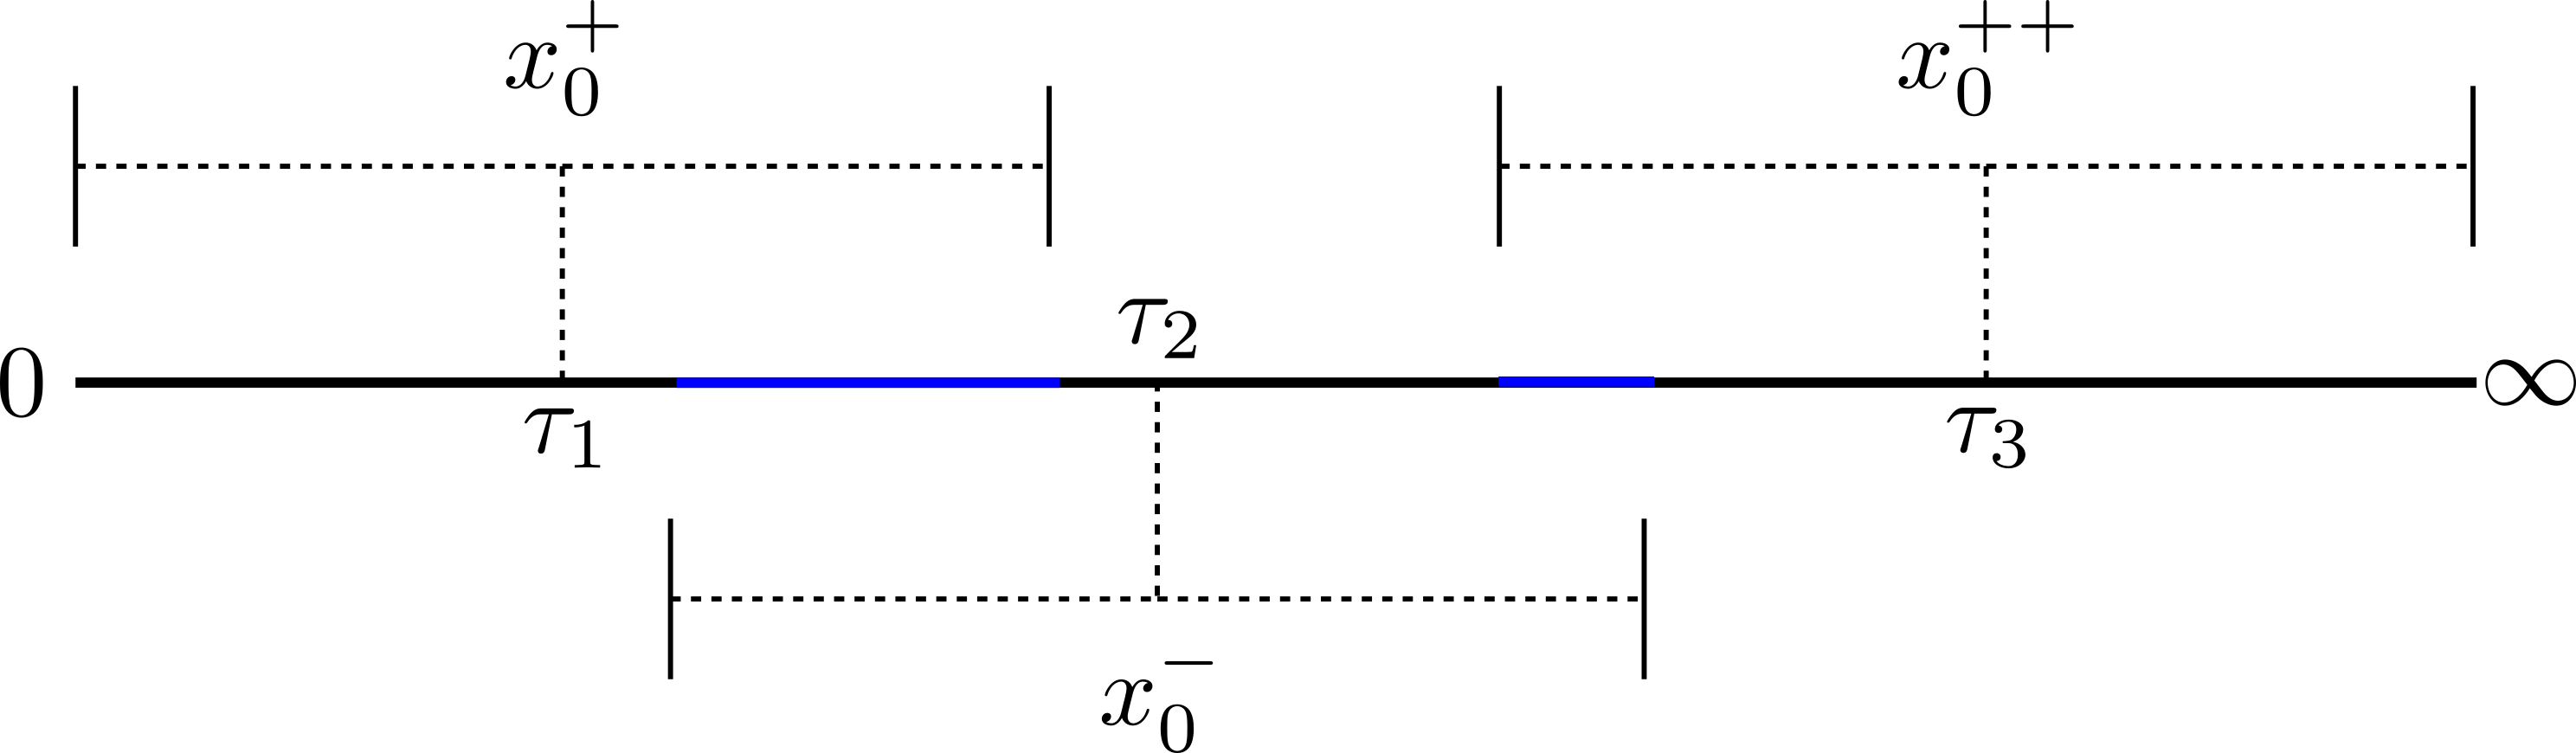
\includegraphics[width=0.8\textwidth]{./instantons.png}
	\caption{Configuration of the function over all time. The blue regions in time involve multiple stationary states overlapping with each other.}
	\label{conf}
\end{figure}
Their are two stretches of time (drawn in blue) where the configuration of the function is a sum of two stationary solutions. Since the potential \(V(x)\) is not necessarily linear, these superposed functions are not in general solutions of the Euler-Lagrange equations. We will, however, approach stationary solutions when the solutions become more separated in time, becoming exact in the limit of \(\tau_2 \gg \tau_1, \)become more and more separated. That is, when  \il{\tau_1 \ll \tau_2 \ll \tau_3}. Then, the total solution will be of the form shown in fig.~\ref{conf2}.
\begin{figure}[htpb!]
	\centering
	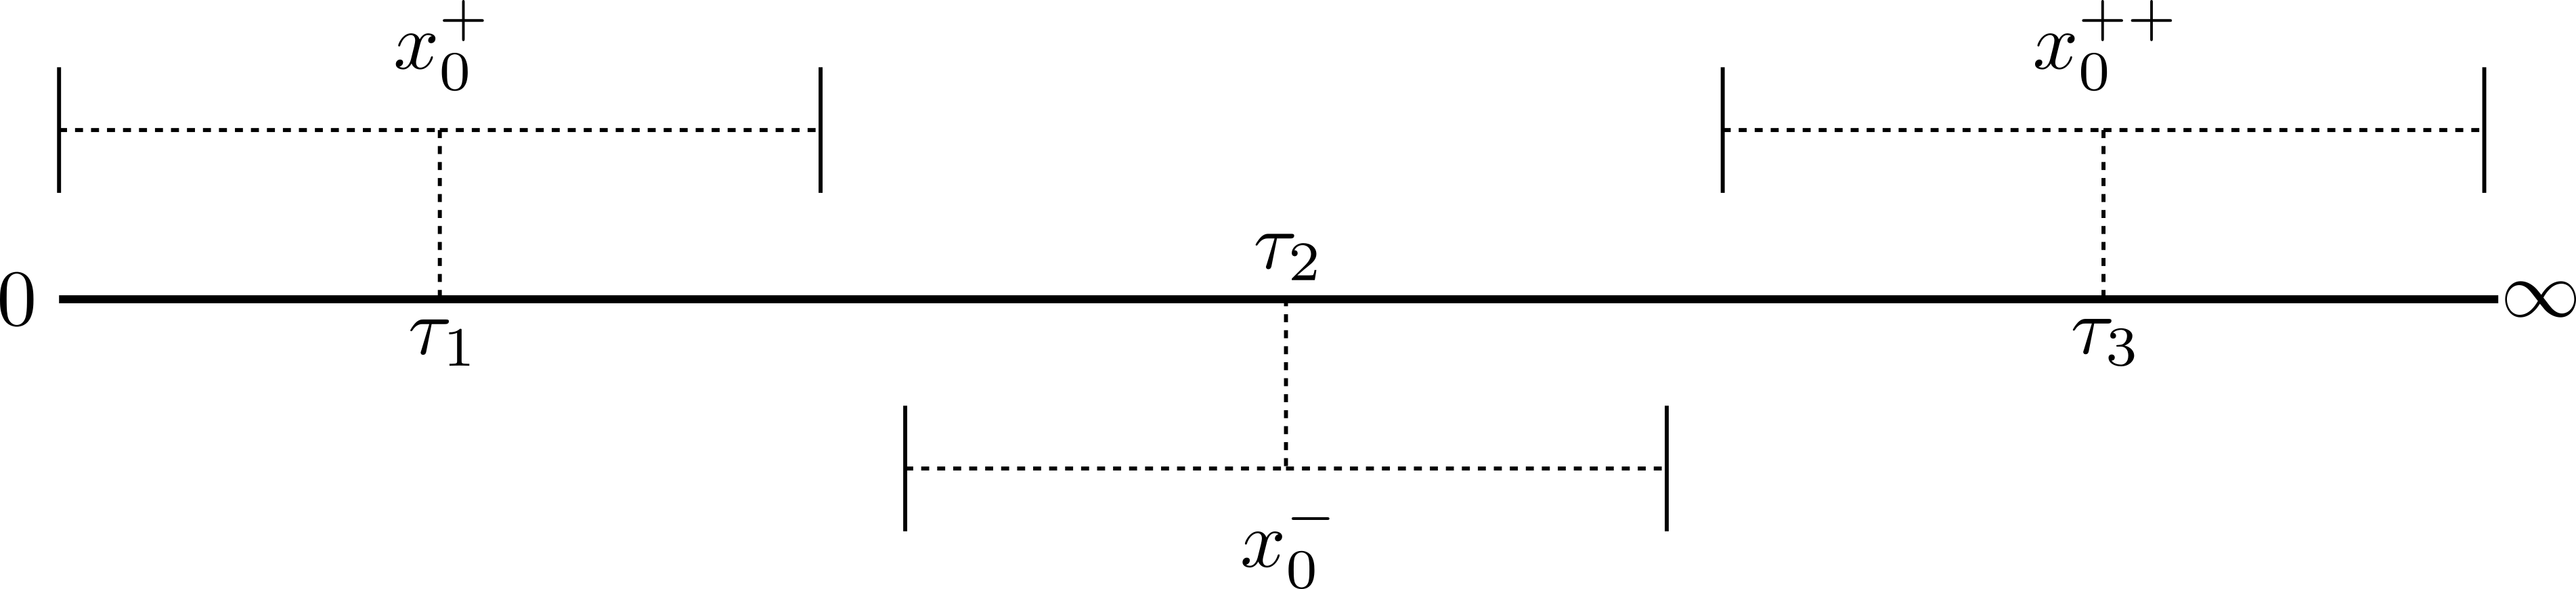
\includegraphics[width=0.8\textwidth]{./instantons2.png}
	\caption{Configuration of (anti-)instantons that are well-separated in time, and hence producing stationary states of the action.}
	\label{conf2}
\end{figure}
In such a configuration we see that at each point, only a single solution enters the minimization equation. This means that in the limit of \il{\tau \ra \infty}, these solutions are possible because then we will be able to set \il{\tau_1 \ll \tau_2}.  The only constraint to maintain the boundary condition is \il{n_1 - n_2 =1}.\\\\
The total contribution coming from \il{n_1} instantons and \il{n_2} anti-instantons is\beq
P_{n_1,n_2} = \fr{\delta_{n_1 - n_2 =1}}{n_1 ! n_2 !}\qq{\sqrt{S_0} \tau e^{-\fr{1}{\hbar}S_0}\mc{K}}^{n_1+n_2}\sqrt{\fr{ \omega  }{\pi \hbar }}e^{-\fr{\omega}{2} \tau}
\eeq
Each solution contributes a prefactor  \il{\sqrt{S_0} \tau e^{-\fr{1}{\hbar}S_0}} due to the individual integrations over  the zero-modes. Each solution also contributes a factor of \il{\mc{K}} because of the individual regions where they are not at the boundaries. The remaining stretches along the time axis where the configuration is near \(0\) or \(a\), for all (anti-)instantons, will give the harmonic oscillator determinant, which as a result comes just once. We have also divided by the total number of permutations of the instantons as well as the anti-instantons, because they are indistinguishable. \\\\
This is for a particular pair of values \il{n_1} and \il{n_2}. We can sum over these values to get the total probability.
\beq[mikasa]
\bra{x=a} e^{-\fr{\tau}{\hbar}H} \ket{0} = \sqrt{\fr{ \omega  }{\pi \hbar }}e^{-\fr{\omega}{2} \tau}\sum_{n_1,n_2}\fr{\delta_{n_1 - n_2 =1}}{n_1 ! n_2 !}\qq{\sqrt{S_0} \tau e^{-\fr{1}{\hbar}S_0}\mc{K}}^{n_1+n_2}
\eeq
We can change the Kronecker-delta to its Fourier transform.
\beq
\delta_{n_1 - n_2 =1} = \int_0^{2\pi}\fr{d\theta}{2\pi}\ex{-i\theta(n_1 - n_2 -1)}
\eeq
Define \il{\gamma = \sqrt{S_0} \tau e^{-\fr{1}{\hbar}S_0}\mc{K}}. The delta Fourier transform gives
\beq
\bra{x=a} e^{-\fr{\tau}{\hbar}H} \ket{0} &= \sqrt{\fr{ \omega  }{\pi \hbar }}e^{-\fr{\omega}{2} \tau}\sum_{n_1,n_2}\int_0^{2\pi}\fr{d\theta}{2\pi}\ex{-i\theta(n_1 - n_2 -1)}\fr{\gamma^{n_1+n_2}}{n_1 ! n_2 !}\\
					  &=\sqrt{\fr{ \omega  }{\pi \hbar }}e^{-\fr{\omega}{2} \tau}\int \fr{d\theta}{2\pi}e^{i\theta} \sum_{n_1} \fr{\rr{\gamma e^{-i\theta}}^{n_1}}{n_1 !}\sum_{n_2} \fr{\rr{\gamma e^{i\theta}}^{n_2}}{n_2 !}\\
					  &=\sqrt{\fr{ \omega  }{\pi \hbar }}e^{-\fr{\omega}{2} \tau}\int \fr{d\theta}{2\pi}e^{i\theta} \ex{2\gamma\cos\theta}\\
					  &=\sqrt{\fr{ \omega  }{\pi \hbar }}\int \fr{d\theta}{2\pi}e^{i\theta} \ex{\fr{\tau}{\hbar}\qq{2\hbar\sqrt{S_0} e^{-\fr{1}{\hbar}S_0}\mc{K}\cos\theta-\fr{\hbar\omega}{2}}}
\eeq
Comparing with eq.~\ref{sasageyo},
\begin{equation}\begin{aligned}
\label{main}
\lim_{\tau \to \infty}\sum_n \avg{x=a|n} e^{-\fr{\tau}{\hbar}E_n} \avg{n|0} = \lim_{\tau \to \infty}\sqrt{\fr{ \omega  }{\pi \hbar }}\int \fr{d\theta}{2\pi}e^{i\theta} \ex{-\fr{\tau}{\hbar}\qq{\fr{\hbar\omega}{2}-2\hbar\sqrt{S_0} e^{-\fr{1}{\hbar}S_0}\mc{K}\cos\theta}}\\
\end{aligned}\end{equation}
\subsection*{Extracting the band dispersion from the total propagator}
For \il{\tau \ra \infty}, the left-hand side will be dominated by the smaller values of \il{E_n}, because the negative exponential will fall very fast for large \il{\tau} and large \il{E_n}. Those same low-lying energy levels are found to form a continuous band on the right hand side. The energy states in this lowest band are parametrised by \il{\theta}. We can hence write
\beq
E_\text{low} \approx E_\theta = \fr{\hbar\omega}{2}-2\hbar\sqrt{S_0} e^{-\fr{1}{\hbar}S_0}\mc{K}\cos\theta
\eeq
and identity \(\theta\) as the dimensionless variable \(ka\), and \il{t = \sqrt{S_0} \tau e^{-\fr{1}{\hbar}S_0}\mc{K}}. Eq.~\ref{Bloch}  can also be reproduced by this method. From eq.~\ref{main}, we can write
\beq[states]
\avg{x=a|k}\avg{k|0} = \sqrt{\fr{ \omega  }{\pi \hbar }}e^{ika}
\eeq
There we assumed we are at the lowest band and the only remaining quantum number is the crystal momentum. Now, we have only considered situations where the net effect of the solution is to go from \il{x=0} to \il{x=a}. If we allowed the instanton to tunnel through \(N\) barriers and reach \il{x=Na}, the boundary condition would require \il{n_1 - n_2 = N}. This means the delta function would become \il{\delta_{n_1 - n_2 - N}}. The corresponding Fourier transform would involve the exponent \il{\ex{-ik\qq{n_1 - n_2 - N}}}, so the only change is  \il{\theta \ra N\theta}. Eq.~\ref{states} will then become
\beq[first]
\avg{Na|k}\avg{k|0} = \sqrt{\fr{ \omega  }{\pi \hbar }}e^{iN ka}
\eeq
Putting \il{N=0} gives
\beq[second]
\avg{0|k}\avg{k|0} = \sqrt{\fr{ \omega  }{\pi \hbar }}
\eeq
Dividing eq.~\ref{first} by eq.~\ref{second} gives
\beq
\avg{Na|k}= e^{iNka}\avg{0|k}
\eeq
We can interpret \il{\avg{Na|k} = \psi_k(Na), \avg{0|\theta} = \psi_\theta(0)}. This means
\beq[guren]
\psi_k(Na) = e^{iNka}\psi_k(0)
\eeq
\subsection*{Mapping the lattice problem to that on a circle: twisted boundary conditions}
If the particle is placed on a ring with the same periodic potential, the Lagrangian remains the same, so the local equation of motion satisfied by the solutions remains the same. But the boundary conditions will change. For the ring, the points \il{x = 0} and \il{x=a} are physically the same, so we must require 
\beq
\psi(x) = \psi(x+a)
\eeq
From the Bloch theorem (eq.~\ref{Bloch}), this means we can only have \il{k=0}, which amounts to taking only the central momentum in the Brillouin zone, per band. Equivalently, from eq.~\ref{guren}, it means we can only have \il{\theta = 0} from the lowest band. Each band thus gets reduced to one state (\il{k=0} or \il{\theta = 0}). To get the other states of the lowest band, we can make a modification to the Lagrangian which does not change the local physics but changes the boundary conditions. We take the new Lagrangian
\beq[newl]
\mc{L}_E^\prime= \fr{1}{2}\dot x^2 + V(x) + i\fr{\hbar\theta}{a}\dot x
\eeq
The extra term is a total derivative (we assume \il{\theta} is a constant). Since this is a total derivative term, the local equations of motion will not change. However, as we will see later, \(\theta\) acts like a vector potential that couples with the velocity. We know from other standard calculations that the presence of such a vector potential term can be removed from the Lagrangian (Hamiltonian) by a large gauge transformation but such a process modifies the boundary conditions: periodic boundary conditions change into twisted boundary conditions.
\begin{equation}\begin{aligned}
	\psi(x+a) = e^{-i\theta}\psi(x) = e^{-ika}\psi(x)
\end{aligned}\end{equation}
The \il{\hbar} is inserted to fix the dimensions. This is just Bloch's theorem, and these twisted boundary conditions show that the effect of the total derivative term with a non-zero \(\theta\) is to introduce the non-zero values of the crystal momentum into the problem by reproducing Bloch's theorem.\\\\
In the presence of this term, the change to the action is
\beq
S_E^\prime &= \int d\tau^\prime \cc{\fr{1}{2}\dot x^2 + V(x) + i\fr{\hbar\theta}{a}\dot x} \\
&= S_E + i\hbar\theta\int \frac{d\tau^\prime}{a}\dot x \\
&= S_E + i\hbar\theta\int_0^{a} \frac{dx}{a} \\ 
&= S_E + i\hbar\theta
\eeq
This was for an instanton because we assumed \il{x} went from \il{0} to \il{a}. For anti-instanton, we will have
\beq
S_E^\prime = S_E + i\theta\int_{a}^0 \frac{dx}{a} = S_E - i\hbar\theta
\eeq
The total contribution from \(n_1\) instantons and \(n_2\) anti-instantons, which previously was \il{\ex{-\fr{S_0}{\hbar}\rr{n_1 + n_2}}}, now becomes
\beq
\ex{-\fr{S_0}{\hbar}\rr{n_1 + n_2}}e^{-i\theta\rr{n_1 - n_2}}
\eeq
One difference from the lattice problem is that here we do not need \il{n_1 - n_2 = 1}. As long as \il{n_1} and \il{n_2} are integers, the total distance traveled  by the solution will be \il{a} times some integer which will always correspond to the point \il{x=0=a}. This means we can drop the Kronecker delta in eq.~\ref{mikasa}, which now becomes
\beq
\bra{a} e^{-\fr{\tau}{\hbar}H} \ket{0} &= \sqrt{\fr{ \omega  }{\pi \hbar }}e^{-\fr{\omega}{2} \tau}\sum_{n_1,n_2}\fr{1}{n_1 ! n_2 !}\qq{\sqrt{S_0} \tau e^{-\fr{1}{\hbar}S_0}\mc{K}}^{n_1+n_2}e^{-i\theta\rr{n_1 - n_2}}\\
					  &=\sqrt{\fr{ \omega  }{\pi \hbar }}e^{-\fr{\omega}{2} \tau}\sum_{n_1}\fr{1}{n_1 !}\qq{\gamma e^{-i\theta}}^{n_1}\sum_{n_2}\fr{1}{n_2 !}\qq{\gamma e^{i\theta}}^{n_2}\\
					  &=\sqrt{\fr{ \omega  }{\pi \hbar }}e^{-\fr{\omega}{2} \tau}\ex{2\gamma \cos \theta}
\eeq
The new energy levels are thus
\beq
E_\theta = \fr{\hbar \omega}{2} - 2 \sqrt{S_0} \tau e^{-\fr{1}{\hbar}S_0}\mc{K} \cos \theta
\eeq
We are thus able to recover the band by choosing various values of \(\theta\).
\subsection*{The crystal momentum as an Aharonov-Bohm flux}
When we introduced the total derivative term into the Lagrangian, we had mentioned briefly that the term acts like a vector potential coupling term. Here will make that more concrete. We can compare the new Lagrangian, eq.~\ref{newl}, to a difference physical setting. Consider a particle on a ring with a periodic potential, with a constant magnetic field \il{B} along \il{\hat z} through the center of the ring. \il{\phi} is the azimuthal coordinate. The Lagrangian for such a charged particle moving in a magnetic field is given by
\begin{equation}\begin{aligned}
	\mathcal{L}^\prime = \mathcal{L} - eA \dot x
\end{aligned}\end{equation}
where \(A\) is the vector potential. For a constant magnetic field, it can be expressed as
\beq
\vec A &= \fr{1}{2}\vec r \times \vec B = \fr{1}{2}Br\hat \phi \implies A(R) &= \frac{\Phi}{a}
\eeq
\il{\Phi = B\pi R^2} is the flux of the magnetic field through the ring, \il{R} being the radius. 
The Euclidean form of this Lagrangian will absorb the minus sign of the additional term.
\begin{equation}\begin{aligned}
	-\mathcal{L}_E^\prime = -\mathcal{L}_E - ieA \frac{\:\mathrm{d}x}{\:\mathrm{d}\tau} \implies \mathcal{L}_E^\prime = \mathcal{L}_E + ieA \frac{\:\mathrm{d}x}{\:\mathrm{d}\tau}
\end{aligned}\end{equation}
Comparing the two changed Lagrangians, we can see that the total derivative term we introduced earlier is equivalent to the vector-potential term (and hence the flux \(\Phi\)).
\beq[sakura]
eA = \fr{\hbar\theta}{a} \implies \theta = \frac{e\Phi}{\hbar}
\eeq
We already know that the crystal momentum is given by \(k = \frac{\theta}{a}\). This then gives
\begin{equation}\begin{aligned}
k = \fr{e\Phi}{a\hbar}
\end{aligned}\end{equation}
\subsection*{Topological nature of the crystal momentum}
The winding number of the particle trajectories is the number of times the particle completes the loop. This number is \(n_1 - n_2\), because the instantons traverse the loop in the forward direction, while the anti-instantons do it in the opposite direction.
\begin{equation}\begin{aligned}
	W = n_1 - n_2
\end{aligned}\end{equation}
Looking back to the lattice problem, we can recognize this quantity as the number of barriers that a general configuration tunnels through. This can also be related to a topological charge. The topological charge of an instanton that has the boundary conditions at \(x = \pm \eta\) is
\begin{equation}\begin{aligned}
	Q \equiv \frac{1}{2\eta}\int \dot x dt = \frac{1}{2\eta}\left(x(\infty) - x(-\infty)\right)
\end{aligned}\end{equation}
The instantons thus have a topological charge of \(Q = 1\), while the anti-instantons have \(Q = -1\). These values are topological invariants; a function with a particular topological charge cannot be smoothly deformed into another. A general configuration of \(n_1\) instantons and \(n_2\) instantons has a topological charge of \(n_1 - n_2\). We thus see that the winding number is the topological charge.
But we also know that \il{n_1} instantons travel a distance of \il{2\pi n_1} on the lattice, and \il{n_2} anti-instantons travel \il{-2\pi n_2}, so that the total distance traveled on the lattice is \il{2\pi\rr{n_1 - n_2}}. Since each lattice spacing is worth \il{2\pi}, the number of lattice spacing traversed also comes out to be \il{n_1 - n_2}. In this way, we can see that the winding quantum number is equivalent to the number of lattice spacing traveled by the instantons.
\begin{equation}\begin{aligned}
	W = n_1 - n_2 = Q
\end{aligned}\end{equation}
From the spectrum of the particle on a circle,
\begin{equation}\begin{aligned}
	E_n \propto (n - \frac{\Phi}{\Phi_0})^2
\end{aligned}\end{equation}
This means that the only values of the flux that keep the physics invariant are integer multiples of the flux quantum \(\Phi_0 = \frac{2\hbar}{e}\). In other words, the flux becomes related to the topological charge \(Q\). This also places a constraint on the crystal momentum \(k\):
\begin{equation}\begin{aligned}
	k = \frac{e}{a\hbar}\Phi_0 Q
\end{aligned}\end{equation}
It is now clearly seen that the crystal momentum is related to the topological charge. Different values of the topological charge are obtained from topologically different functions, and lead to different values of the crystal momentum.
\begin{appendices}
\subsection*{Appendix: Evaluation of the integral}
We divide the time range and position ranges into \il{N} slices, each slice of width \il{\Delta \tau = \fr{\tau}{N}} (\il{\Delta x = \fr{2\pi}{N}}). We get a sequence of discrete points, \il{\tau_m = -\fr{\tau}{2}+m\Delta \tau}. Similarly \il{x_m = 0 + m\Delta x}. Obviously \il{\tau_0 = -\fr{\tau}{2}} and \il{\tau_N = \fr{\tau}{2}}. Then, 
\beq
U(\fr{\tau}{2},-\fr{\tau}{2})=e^{-\fr{\tau}{\hbar}H} = \prod_{m=0}^{N-1} U(\tau_m+1, \tau_{m})
\eeq
The term \il{U_m \equiv U(\tau_m, \tau_{m+1})} can be approximated as
\beq
U_m = \text{exp}\qq{-\fr{\Delta\tau}{\hbar}\rr{H_0 + V}} &= e^{-\fr{\Delta\tau}{\hbar}H_0}e^{-\fr{\Delta\tau}{\hbar}V}\qq{1+O(\Delta\tau^2)}\\
			       &\approx e^{-\fr{\Delta\tau}{\hbar}H_0}e^{-\fr{\Delta\tau}{\hbar}V}
\eeq
Noting that \il{\int dx_m \ket{x_m}\bra{x_m} = 1}, we can write the following.
\beq
\bra{2\pi} e^{-\fr{\tau}{\hbar}H} \ket{0} = \prod_{m=0}^{N-1} \bra{2\pi} U(\tau_m, \tau_{m+1})\ket{0} = \prod_{m=N-1}^{0}\int_{-\infty}^\infty dx_m \bra{x_{m+1}} U(\tau_m, \tau_{m+1})\ket{x_m}
\eeq
The \il{m^\text{th}} inner product can be evaluated easily.
\beq
\bra{x_{m+1}} U(\tau_m, \tau_{m+1})\ket{x_m} &= \bra{x_{m+1}} \ex{-\fr{\Delta \tau}{\hbar}H_0}\ket{x_m}\ex{-\fr{\Delta \tau}{\hbar}V(x_m)}\\
					     &=\mathcal{M} \ex{\fr{-1}{2\hbar\Delta \tau}\rr{x_{m+1} - x_m}^2}\ex{-i\fr{\Delta \tau}{\hbar}V(x_m)}\\
					     &=\mathcal{M} \text{exp}\qq{\fr{-\Delta\tau}{\hbar}\cc{\fr{1}{2}\rr{\fr{x_{m+1} - x_m}{\Delta \tau}}^2 + V(x_m)}}\\
\eeq
\il{\mathcal{M}} is a factor that will be absorbed later so we won't bother with it. Now we take the limit of \il{N \ra \infty}. This makes
\begin{gather}
\tau_m \ra \tau^\prime\\
\Delta \tau \ra d\tau^\prime\\
x_m(\tau_m) \ra x(\tau^\prime)\\
x_{m+1} - x_m = \Delta x_m(\tau_m) \ra dx
\end{gather}
We thus get the following in that limit.
\beq
\bra{x_{m+1}} U(\tau_m, \tau_{m+1})\ket{x_m} =\mathcal{M} \text{exp}\qq{\fr{-d\tau^\prime}{\hbar}\cc{\fr{1}{2}\dot x^2 + V(x)}}\\
\eeq
where \il{\dot x = \dv{x(\tau^\prime)}{\tau^\prime}}. The final result is
\beq
\bra{2\pi} e^{-\fr{\tau}{\hbar}H} \ket{0} &=\int_{-\infty}^\infty \prod_{m=N-1}^{0}dx_m \mathcal{M}^N \ex{-\fr{1}{\hbar}\int_{-\fr{\tau}{2}}^{\fr{\tau}{2}} d\tau^\prime \cc{\fr{1}{2}\dot x^2 + V(x)}}\\
					  &=\int\mathcal{D}\qq{x(\tau^\prime)}\ex{-\fr{S_E\qq{x(\tau^\prime)}}{\hbar}}
\eeq

\end{appendices}
\end{document}
